%%%%%%%%%%%%%%%%%%%%%%%%%%%%%%%%%%%%%%%%%
% Masters/Doctoral Thesis 
% LaTeX Template
% Version 2.1 (2/9/15)
%
% This template has been downloaded from:
% http://www.LaTeXTemplates.com
%
% Version 2.0 major modifications by:
% Vel (vel@latextemplates.com)
%
% Original authors:
% Steven Gunn  (http://users.ecs.soton.ac.uk/srg/softwaretools/document/templates/)
% Sunil Patel (http://www.sunilpatel.co.uk/thesis-template/)
%
% License:
% CC BY-NC-SA 3.0 (http://creativecommons.org/licenses/by-nc-sa/3.0/)
%
%%%%%%%%%%%%%%%%%%%%%%%%%%%%%%%%%%%%%%%%%

%----------------------------------------------------------------------------------------
%	PACKAGES AND OTHER DOCUMENT CONFIGURATIONS
%----------------------------------------------------------------------------------------

\documentclass[
11pt, % The default document font size, options: 10pt, 11pt, 12pt
%oneside, % Two side (alternating margins) for binding by default, uncomment to switch to one side
brazilian, % ngerman for German
singlespacing, % Single line spacing, alternatives: onehalfspacing or doublespacing
%draft, % Uncomment to enable draft mode (no pictures, no links, overfull hboxes indicated)
%nolistspacing, % If the document is onehalfspacing or doublespacing, uncomment this to set spacing in lists to single
%liststotoc, % Uncomment to add the list of figures/tables/etc to the table of contents
%toctotoc, % Uncomment to add the main table of contents to the table of contents
%parskip, % Uncomment to add space between paragraphs
]{MastersDoctoralThesis} % The class file specifying the document structure

\usepackage[utf8]{inputenc} % Required for inputting international characters
\usepackage[T1]{fontenc} % Output font encoding for international characters

\usepackage{palatino} % Use the Palatino font by default

\usepackage[backend=bibtex,style=authoryear,natbib=true]{biblatex} % User the bibtex backend with the authoryear citation style (which resembles APA)

\addbibresource{main.bib} % The filename of the bibliography

\usepackage[autostyle=true]{csquotes} % Required to generate language-dependent quotes in the bibliography
\usepackage{amssymb}
\usepackage{amsmath}
\usepackage{hyperref}
\usepackage{algorithm}
\usepackage[noend]{algpseudocode}
\usepackage{hyperref}
\usepackage{enumitem}
%\usepackage[]{algorithm2e}
%\usepackage{algorithmic}
%\usepackage[colorlinks=true,linkcolor=blue]{hyperref} 

\newtheorem{theorem}{Teorema}
\newtheorem{definition}{Definição}
\newtheorem{proof}{Demonstracão}
\newtheorem{corollary}{Corolário}
\newtheorem{proposition}{Proposição}

\makeatletter
\def\BState{\State\hskip-\ALG@thistlm}
\makeatother


%----------------------------------------------------------------------------------------
%	THESIS INFORMATION
%----------------------------------------------------------------------------------------

\thesistitle{Teoria dos Números e Computação: Uma abordagem utilizando problemas de competições de programação} % Your thesis title, this is used in the title and abstract, print it elsewhere with \ttitle
\supervisor{Dr. Carlos Eduardo Ferreira} % Your supervisor's name, this is used in the title page, print it elsewhere with \supname
\examiner{} % Your examiner's name, this is not currently used anywhere in the template, print it elsewhere with \examname
\degree{Bacharel em Ciência da Computação} % Your degree name, this is used in the title page and abstract, print it elsewhere with \degreename
\author{Antonio R. de Campos Junior} % Your name, this is used in the title page and abstract, print it elsewhere with \authorname
\addresses{} % Your address, this is not currently used anywhere in the template, print it elsewhere with \addressname

\subject{Ciência da Computação} % Your subject area, this is not currently used anywhere in the template, print it elsewhere with \subjectname
\keywords{} % Keywords for your thesis, this is not currently used anywhere in the template, print it elsewhere with \keywordnames
\university{\href{http://www5.usp.br/}{Universidade de São Paulo}} % Your university's name and URL, this is used in the title page and abstract, print it elsewhere with \univname
\department{\href{http://www.ime.usp.br/}{Instituto de Matemática e Estatística}} % Your department's name and URL, this is used in the title page and abstract, print it elsewhere with \deptname
\group{\href{http://researchgroup.university.com}{Research Group Name}} % Your research group's name and URL, this is used in the title page, print it elsewhere with \groupname
\faculty{\href{http://faculty.university.com}{Faculty Name}} % Your faculty's name and URL, this is used in the title page and abstract, print it elsewhere with \facname

\hypersetup{pdftitle=\ttitle} % Set the PDF's title to your title
\hypersetup{pdfauthor=\authorname} % Set the PDF's author to your name
\hypersetup{pdfkeywords=\keywordnames} % Set the PDF's keywords to your keywords

\begin{document}

\frontmatter % Use roman page numbering style (i, ii, iii, iv...) for the pre-content pages

\pagestyle{plain} % Default to the plain heading style until the thesis style is called for the body content

%----------------------------------------------------------------------------------------
%	TITLE PAGE
%----------------------------------------------------------------------------------------

\begin{titlepage}
\begin{center}

\textsc{\LARGE \univname}\\[1.5cm] % University name
\textsc{\Large Trabalho de Formatura}\\[0.5cm] % Thesis type

\HRule \\[0.4cm] % Horizontal line
{\huge \bfseries \ttitle}\\[0.4cm] % Thesis title
\HRule \\[1.5cm] % Horizontal line
 
\begin{minipage}{0.4\textwidth}
\begin{flushleft} \large
\emph{Autor:}\\
\href{http://www.ime.usp.br/~arcjr}{\authorname} % Author name - remove the \href bracket to remove the link
\end{flushleft}
\end{minipage}
\begin{minipage}{0.4\textwidth}
\begin{flushright} \large
\emph{Supervisor:} \\
\href{http://www.ime.usp.br/~cef/}{\supname} % Supervisor name - remove the \href bracket to remove the link  
\end{flushright}
\end{minipage}\\[3cm]
\leavevmode \\
\leavevmode \\
\leavevmode \\
\leavevmode \\

\large \textit{Tese apresentada em cumprimento dos requisitos para o curso \\ \degreename}\\[0.3cm] % University requirement text
%\textit{in the}\\[0.4cm]
\deptname\\[2cm] % Research group name and department name
 
{\large \today}\\[4cm] % Date
%\includegraphics{Logo} % University/department logo - uncomment to place it
 
\vfill
\end{center}
\end{titlepage}

%----------------------------------------------------------------------------------------
%	DECLARATION PAGE
%----------------------------------------------------------------------------------------

%----------------------------------------------------------------------------------------
%	QUOTATION PAGE
%----------------------------------------------------------------------------------------

\vspace*{0.2\textheight}

\noindent\enquote{\itshape To raise new questions, new possibilities, to regard old problems from a new angle, requires creative imagination and marks real advance in science.}\bigbreak

\hfill Albert Einstein
\newpage
%----------------------------------------------------------------------------------------
%	ABSTRACT PAGE
%----------------------------------------------------------------------------------------

\chapter*{Resumo}
\thispagestyle{empty}

Teoria do Números é um vasto ramo da matemática que estuda números inteiros. Números primos, fatorização de números inteiros, funções aritméticas, são alguns dos tópicos mais estudados e também importantes para resolução de problemas computacionais.

Hoje em dia a importância da Teoria do Números na Computação é inquestionável, e desse modo, esse trabalho vem ilustrar como a teoria pode ser aplicada na criação de algoritmos para resolução de problemas computacionais, em especial problemas de competições de programação.

Equações diofantinas, Congruência Modular, Números de Fibonacci, são alguns dos assuntos que serão abordados nesse trabalho. Após a devida demostração da teoria serão exibidos alguns problemas de competições de programação que aplicam essa teoria, seguido da implementação e análise do algoritmo que resolve o problema abordado.

\clearpage

%\section{abstract}
%\addchaptertocentry{\abstractname} % Add the abstract to the table of contents

%The Thesis Abstract is written here (and usually kept to just this page). The page is kept centered vertically so can expand into the blank space above the title too\ldots

%\end{abstract}

%----------------------------------------------------------------------------------------
%	ACKNOWLEDGEMENTS
%----------------------------------------------------------------------------------------

\chapter*{Agradecimentos}
\thispagestyle{empty}
Gostaria de agradecer ao doutorando \textit{Renzo Gonzalo Gomez Diaz} pelo auxílio na revisão dos textos e na seleção dos problemas.
E um agradecimento especial ao Professor Doutor \textit{Carlos Eduardo Ferreira} pelo suporte durante todo o desenvolvimento desse trabalho.
%I like to acknowledge ...

\clearpage
%\section{acknowledgements}
%\addchaptertocentry{\acknowledgementname} % Add the acknowledgements to the table of contents

%The acknowledgements and the people to thank go here, don't forget to include your project advisor\ldots

%\end{acknowledgements}

%----------------------------------------------------------------------------------------
%	LIST OF CONTENTS/FIGURES/TABLES PAGES
%----------------------------------------------------------------------------------------

\tableofcontents % Prints the main table of contents

%\listoffigures % Prints the list of figures

%\listoftables % Prints the list of tables

%----------------------------------------------------------------------------------------
%	ABBREVIATIONS
%----------------------------------------------------------------------------------------

%\section{abbreviations}{ll} % Include a list of abbreviations (a table of two columns)

%\textbf{LAH} & \textbf{L}ist \textbf{A}bbreviations \textbf{H}ere\\
%\textbf{WSF} & \textbf{W}hat (it) \textbf{S}tands \textbf{F}or\\

%\end{abbreviations}

%----------------------------------------------------------------------------------------
%	PHYSICAL CONSTANTS/OTHER DEFINITIONS
%----------------------------------------------------------------------------------------

%\section{constants}{lr@{${}={}$}l} % The list of physical constants is a three column table

% The \SI{}{} command is provided by the siunitx package, see its documentation for instructions on how to use it

%Speed of Light & $c$ & \SI{2.99792458e8}{\meter\per\second} (exact)\\
%Constant Name & $Symbol$ & $Constant Value$ with units\\

%\end{constants}

%----------------------------------------------------------------------------------------
%	SYMBOLS
%----------------------------------------------------------------------------------------

%\section{symbols}{lll} % Include a list of Symbols (a three column table)

%$a$ & distance & \si{\meter} \\
%$P$ & power & \si{\watt} (\si{\joule\per\second}) \\
%Symbol & Name & Unit \\

%\addlinespace % Gap to separate the Roman symbols from the Greek

%$\omega$ & angular frequency & \si{\radian} \\

%\end{symbols}

%----------------------------------------------------------------------------------------
%	DEDICATION
%----------------------------------------------------------------------------------------

%\dedicatory{For/Dedicated to/To my\ldots} 

%----------------------------------------------------------------------------------------
%	THESIS CONTENT - CHAPTERS
%----------------------------------------------------------------------------------------

\mainmatter % Begin numeric (1,2,3...) page numbering

\pagestyle{thesis} % Return the page headers back to the "thesis" style

% Include the chapters of the thesis as separate files from the Chapters folder
% Uncomment the lines as you write the chapters

% Chapter 1

\chapter{Divisibilidade} % Main chapter title

\label{Chapter1} % Change X to a consecutive number; for referencing this chapter elsewhere, use \ref{ChapterX}

%----------------------------------------------------------------------------------------
%	SECTION 1
%----------------------------------------------------------------------------------------

\section{Introdução}
A noção de divisibilidade dos números inteiros é fundamental na \textbf{Teoria dos Números}.
Nesse seção vamos descrever algumas definições e propriedades que serão utilizados ao longo desse trabalho.

\begin{definition}
A notação $d|n$ ("$d$ \textbf{divive} $n$"), significa que existe um inteiro $q$, tal que, $n = dq$.
Se $d|n$ dizemos que $n$ é múltiplo de $d$. Caso $n$ não seja múltiplo de $d$ (ou seja, $d$ não divide $n$), escrevemos $d \nmid n$.
\end{definition}


\begin{corollary}\label{divisibilidade_transitiva}
$d|n$ , $d|m \Rightarrow d|(n+m)$
\end{corollary}
\textbf{Demonstração:}
Se $d|n$ e $d|m$, então existe inteiros $q$ e $k$, tal que, $n = qd$ e $m = kd$. Desse modo temos:

$(n+m) = qd + kd = (q + k)d \Rightarrow d|(n+m) $ $\square$


\begin{corollary}\label{divisibilidade_fracao}
$d|(\frac{n}{m}) \Rightarrow dm|n$
\end{corollary}
\textbf{Demonstração:}

$d|(\frac{n}{m}) \Rightarrow \exists q \in \mathbb{Z} \mid \frac{n}{m} = qd$

$d|(\frac{n}{m}) \Rightarrow n = q(dm) \Rightarrow dm|n$ $\square$


\begin{corollary}\label{corolario_divisibilidade_1}
Dado um subconjunto dos inteiros $S = \{S_1, S_2, S_3, ..., S_n\}$ ordenado crescentemente, e um número inteiro $d$, tal que, $d|(S_i-S_{i-1})$, $2 \leq i \leq n$, 
temos que: 

$d|(S_i-S_j)$, $\forall S_i, S_j \in S$.

\end{corollary}
\textbf{Demonstração:}
Tome $S_i,S_j \in S$ quaisquer, e sem perda de generalidade assuma que $S_i \geq S_j$ (ie, $i \geq j$, pois $S$ está ordenado crescentemente).

Como $i \geq j$, tome $r \in \mathbb{N}$ como sendo a diferença entre $i$ e $j$ : $i = j + r$.

Vamos agora provar por indução que $d|(S_{j+r}-S_j)$.

Para $r=0$ ou $r=1$ a demostração segue trivialmente.

Assuma que o corolário funciona para $(r-1)$, ie, $d|(S_{j+r-1}-S_j)$. 

Temos então que: 

$d|(S_{j+r}-S_{j+r-1}) \Rightarrow d|(S_{j+r}-S_{j+r-1})+(S_{j+r-1}-S_j)$ ($\triangleright$ \textbf{Corolário} \autoref{divisibilidade_transitiva})

$d|(S_{j+r}-S_{j+r-1}) \Rightarrow d|(S_{j+r}-S_j)$ $\square$ 


\begin{corollary}
O \textbf{Corolário} \autoref{corolario_divisibilidade_1} funciona mesmo se o conjunto $S$ não estiver ordenado.
\end{corollary}
\textbf{Demonstração:}
Deixaremos a demostração a cargo do leitor.


\begin{theorem}[Teorema da Divisão]\label{algoritmo_divisao}
Para todo número inteiro $a$ e qualquer número inteiro positivo $n$, existe inteiros únicos $q$ e $r$, tal que:

$a = qn + r$, $0 \leq r < n$

O valor $q$ ($q = \lfloor  \frac{a}{n} \rfloor$) é chamado de \textbf{quociente} da divisão, e o valor $r$ ($r = a \bmod n$) é chamado de \textbf{resto}
(ou \textbf{resíduo}) da divisão.
\end{theorem}
\textbf{Demonstração:}
Suponha que $q$ e $r$ não sejam únicos, ie, que exista $q^*$ e $r^*$ tal que: $a = q^*n + r^*, 0 \leq r^* < n$.

$a = qn + r = q^*n + r^* \Rightarrow (r - r^*) = (q^* - q)n \Rightarrow (r - r^*) \equiv (q^* - q)n \equiv 0 (mod$ $n)$

Porém, como $r \neq r^*$, e tanto $r$ quanto $r^*$ são menores que $n$, temos que: 

$r \not\equiv r^* (mod$ $n) \Rightarrow (r - r^*) \not\equiv 0 (mod$ $n)$

Chegando numa contradição, e assim $q$ e $r$ são únicos $\square$ \\

\begin{corollary}\label{divisibilidade_modular}
$d|n$ , $d|m \Rightarrow d|(n \bmod m)$
\end{corollary}
\textbf{Demonstração:}

$d|n \Rightarrow n = k_1d, k_1 \in \mathbb{Z}$

$d|m \Rightarrow m = k_2d, k_2 \in \mathbb{Z}$

$n = qm + (n \bmod m) \Rightarrow (n \bmod m) = n - qm$ ($\triangleright$ \autoref{algoritmo_divisao})

$(n \bmod m) = k_1d - qk_2d = (k_1 - qk_2)d \Rightarrow d|(n \bmod m)$ $\square$


\begin{corollary}\label{divisibilidade_modular2}
$d|m$ , $d|(n \bmod m) \Rightarrow d|n$
\end{corollary}
\textbf{Demonstração:}

$d|m \Rightarrow m = k_1d, k_1 \in \mathbb{Z}$

$d|(n \bmod m) \Rightarrow (n \bmod m) = k_2d, k_2 \in \mathbb{Z}$

$n = qm + (n \bmod m) \Rightarrow n = qk_1d + k_2d$ ($\triangleright$ \autoref{algoritmo_divisao})

$n = (qk_1 + k_2)d \Rightarrow d|n$ $\square$


\subsection{Divisores}
Nessa subsessão mostraremos um algoritmo simples para calcular todos os divisores de um determinado número inteiro positivo qualquer.

\begin{theorem} 
O número de divisores de $n \in \mathbb{Z}^{+}$ é da ordem de $O(\sqrt{n})$.
\end{theorem}
\textbf{Demonstração:}
Tome um divisor $d$ de $n$ qualquer, com $d > \sqrt{n}$. Dessa forma sabemos que existe um inteiro $q$, com $n=qd$ (observe que $q$ também é divisor de $n$). 
Como $d > \sqrt{n}$ então $q < \sqrt{n}$. Assim, para qualquer divisor $d$ de $n$ maior que $\sqrt{n}$, existe exatamente um divisor $q$ de $n$ menor que $\sqrt{n}$ correspondente ao mesmo.
O que implica que só existe no máximo $\sqrt{n}$ divisores maiores que $\sqrt{n}$. Por outro lado, claramente só existem $\sqrt{n}$ divisores menores que $\sqrt{n}$.
Concluímos então que o número total de divisores de $n$ é da ordem de $O(\sqrt{n})$. $\square$
\\

\textbf{Pseudocódigo:}
\begin{algorithm}
\caption{Encontra todos os divisores de N}\label{encontra_divisores}
\begin{algorithmic}[1]
\Procedure{FindDivisors (N)}{}
\State $D \gets \emptyset$ \Comment{Conjunto $D$ contém os divisores de $N$}

\For {($d = 1 \text{; } d^2 \leq N \text{; } d++)$}

\If {$d\nmid N$}
\State \textbf{continue}
\EndIf
\State $D \gets D \cup \{d\}$
\State $q \gets \frac{N}{d}$
\If {$q\neq d$}
\State $D \gets D \cup \{q\}$
\EndIf

\EndFor

\State \Return{$D$}
\EndProcedure
\end{algorithmic}
\end{algorithm}

\textbf{Análise:}
O laço da linha 3 consome tempo  $O(\sqrt{N})$, testando se os números menores que $\sqrt{N}$ são divisores. Na linha 7 são calculados os divisores correspondentes maiores 
que $\sqrt{N}$. E a condição da linha 8 garante que se $N$ for quadrado perfeito, então é inserido $\sqrt{N}$ somente uma vez no conjunto $D$.
Assim a complexidade total do algoritmo é $O(\sqrt{N})$.




%-----------------------------------
%	SECTION 2
%-----------------------------------
\section{Números Primos}

\begin{definition} 
Todo número inteiro n (n > 1) que têm apenas dois divisores distintos (1 e n) é chamado de número primo. Se n (n > 1) não for primo, dizemos que n é número composto.
\end{definition}


\begin{theorem}[Fatoração Única]\label{fatoracao_unica}
Um número natural qualquer $n$, pode ser escrito unicamente como um produto da forma: 
$n = p_1^{a_1}p_2^{a_2}...p_k^{a_k}$, onde os $p_i$ são números primos, $p_1 < p_2 < ... < p_k$, e os números $a_i$ são inteiros positivos.
\end{theorem}
\textbf{Demonstração:}
Deixaremos a demostração a cargo do leitor.
\textbf{Dica:} Use o fato de que o conjunto dos primos que divide um número inteiro é único, e fato de que se qualquer potência $a_i$ for alterado o valor de $n$ será alterado.



%-----------------------------------
%	SECTION 3
%-----------------------------------
\section{Máximo Divisor Comum}

\begin{definition}
O Máximo Divisor Comum de dois inteiros quaisquer $a$ e $b$ (com a ou b diferente de zero), denotado por $MDC(a,b)$, é o maior inteiro que divide ambos $a$ e $b$. 
Se $MDC(a,b) = 1$ dizemos que $a$ e $b$ são primos entre si.
\end{definition}


\begin{corollary}\label{gcd_modular}
Para números inteiros quaisquer $a$ e $b$, $MDC(a,b) = MDC(b, a \bmod b)$
\end{corollary}
\textbf{Demonstração:}
Pelo \textbf{Corolário} \autoref{divisibilidade_modular} e \autoref{divisibilidade_modular2}, temos:

$d|a, d|b \Leftrightarrow d|b, d|(a \bmod b)$

Assim, qualquer divisor de $a$ e $b$ é também divisor de $b$ e $(a \bmod b)$ (e vise versa). Implicando que o \textbf{Máximo Divisor Comum} de $a$ e $b$
é igual ao \textbf{Máximo Divisor Comum} de $b$ e $(a \bmod b)$. $\square$



\begin{corollary}\label{divisibilidade_mdc}
$MDC(a,b) = d \Rightarrow MDC(\frac{a}{d}, \frac{b}{d}) = 1$
\end{corollary}
\textbf{Demonstração:}
Suponha que $MDC(\frac{a}{d}, \frac{b}{d}) = r > 1$. Assim temos:

$r|\frac{a}{d} \Rightarrow dr|a$ ($\triangleright$ \textbf{Corolário} \autoref{divisibilidade_fracao})

$r|\frac{b}{d} \Rightarrow dr|b$ ($\triangleright$ \textbf{Corolário} \autoref{divisibilidade_fracao})

$r > 1 \Rightarrow dr > d \Rightarrow dr > MDC(a,b)$

Chegamos então numa contradição, pos $dr$ é divisor comum de $a$ e $b$, e $dr$ é maior que o \textbf{Máximo Divisor Comum} de $a$ e $b$. $\square$



\begin{corollary}\label{corolario_gcd_soma}
Para números inteiros quaisquer $a$ e $b$, $MDC(a,b) = MDC(a,a \pm b)$
\end{corollary}
\textbf{Demonstração:}
A prova dessa expressão vem do fato de que qualder divisor de $a$ e $b$, é também divisor de $(a \pm b)$.



\begin{corollary}\label{corolario_gcd_produto}
Para números inteiros quaisquer $a$ e $b$, temos:

$MDC(a,b) = 1 \Rightarrow MDC(a,bk) = MDC(a,k)$, com $k \in \mathbb{Z}$
\end{corollary}
\textbf{Demonstração:}
A prova dessa expressão vem do fato de que qualder divisor $d$ de $a$ e $bk$, é também divisor de $k$, pois $d$ não divide $b$ ($MDC(a,b) = 1$).




\subsection{Algoritmo de Euclides}
A ideia principal do \textbf{Algoritmo de Euclides} é calcular recursivamente o \textbf{Máximo Divisor Comum} de dois números baseando-se no 
\textbf{Corolário} \autoref{gcd_modular}.\\

\textbf{Pseudocódigo:}
\begin{algorithm}
\caption{Algoritmo de Euclides}\label{mdc}
\begin{algorithmic}[1]
\Procedure{$MDC (a, b)$}{}
\If {$b = 0$}
\State \Return $a$
\Else
\State \Return $MDC(b, a \bmod b)$
\EndIf
\EndProcedure
\end{algorithmic}
\end{algorithm}




\subsection{Teorema de Bézout}

\begin{corollary}\label{bezout_conjunto_nao_nulo}
Dado o conjunto de combinações lineares positivas $S := \{x\in\mathbb{Z}, x>0 \mid x = ma + nb, m,n\in \mathbb{Z}\}$, onde os números $a$ e $b$ são inteiros, 
e pelo menos um desses números é diferente de zero. Temos então que $S \neq \emptyset$. 
\end{corollary}
\textbf{Demonstração:}
As combinações possíveis para $a$ e $b$ são:

$a > 0 \Rightarrow |a| = 1.a + 0.b$

$a < 0 \Rightarrow |a| = (-1).a + 0.b$

$b > 0 \Rightarrow |b| = 0.a + 1.b$

$b < 0 \Rightarrow |b| = 0.a + (-1).b$

Como não temos ambos $a$ e $b$ iguais à zero, então $S$ deve conter pelo menos $|a|$ ou $|b|$, e assim $S \neq \emptyset$ $\square$


\begin{corollary}\label{bezout_conjunto_divide}
Dado o conjunto de combinações lineares positivas $S := \{x\in\mathbb{Z}, x>0 \mid x = ma + nb, m,n\in \mathbb{Z}\}$, onde os números $a$ e $b$ são inteiros, 
e pelo menos um desses números é diferente de zero. Temos então que o menor número $d \in S$ divide todos elementos de $S$.
\end{corollary}
\textbf{Demonstração:}
Como $d \in S$, $\exists m,n\in\mathbb{Z} \mid d = ma + nb$.

Tome $x \in S$ qualquer. Pelo \autoref{algoritmo_divisao} $x = qd + r$, $0 \leq r < d$.

Suponha que $d\nmid x$, ie, $x \neq qd$ e $0 < r$. Como $x \in S$, $\exists m^*,n^*\in\mathbb{Z} \mid x = m^*a + n^*b$, e assim:

$x = m^*a + n^*b, x = qd + r \Rightarrow r = m^*a + n^*b - qd = m^*a + n^*b - q(ma + nb)$ 

$\Rightarrow r = (m^* - qm)a + (n^* - qn)b \Rightarrow r \in S$, pois $r > 0$

Chegando numa contrdição, pois $r \in S$, $d \in S$, $r < d$ e $d$ é o menor elemento em $S$.

Desse modo, temos que $d$ divide todos os elementos de $S$. $\square$


\begin{theorem}[Teorema de Bézout]\label{teorema_bezout}
$\forall$ $a$, $b \in \mathbb{Z}$ (com pelo menos um dos dois números diferente de zero), $\exists$ $x, y \in \mathbb{Z} \mid ax + by = mdc(a, b).$
\end{theorem}
\textbf{Demonstração:}
Tome o conjunto das combinações lineares de $a$ e $b$:

$S := \{x\in\mathbb{Z}, x>0 \mid x = ma + nb, m,n\in \mathbb{Z}\}$.

Pelo \textbf{Corolário} \autoref{bezout_conjunto_nao_nulo} sabemos que $S \neq \emptyset$. Como $S$ contém somente números positivos e não é vazio, 
$S$ está limitado inferiormente por \textit{zero} e assim, $S$ tem um elemento mínimo que chamaremos de $d$.

Como $d \in S$, então existe $u, v\in \mathbb{Z}$, tal que, $d = ua + vb$. Pelo \textbf{Corolário} \autoref{bezout_conjunto_divide}, sabemos que $d$ divide todos elementos em $S$, em particular:

$d$ divide $|a|$ e $|b| \Rightarrow d|MDC(a,b) \Rightarrow 0 < d \leq MDC(a,b)$

Por outro lado, $MDC(a,b)$ também divide $a$ e $b$:

$MDC(a,b)|a$ e $MDC(a,b)|b \Rightarrow MDC(a,b)|(ua + vb)$

$ \Rightarrow MDC(a,b)|d \Rightarrow MDC(a,b) \leq d$

$MDC(a,b)\leq d$ e $d \leq MDC(a,b) \Rightarrow MDC(a,b) = d \Rightarrow MDC(a,b) \in S$ $\square$



%----------------------------------------------------------------------------------------
%	SECTION
%----------------------------------------------------------------------------------------

\section{Crivo de Erastóteles}

O \textit{Crivo de Erastótenes} é um algoritmo criado pelo matemático \textbf{Erastótenes} (a.C. 285-194 a.C.) para o cálculo de números primos
até um certo valor limite $N$.
O algoritmo mantém uma tabela com $N$ elementos, e para cada primo, começando pelo número $2$, marca na tabelo os números compostos múltiplos desses primos.
Desse modo, ao final do algoritmo, os elementos não marcados são números primos.\\

\textbf{Pseudocódigo:}
\begin{algorithm}
\caption{Crivo de Erastótenes paro o cálculo de números primos}\label{crivo_erastotenes}
\begin{algorithmic}[1]
\Procedure{CrivoErastótenes (N)}{}
\State $isPrime[] \gets \text{new Array}[N]$ \Comment{$isPrime[]$ é um vetor booleano}

\For {($p = 2 \text{; } p \leq N \text{; } p++)$}
\State $isPrime[p] \gets true$
\EndFor

\For {($p = 2 \text{; } p^2 \leq N \text{; } p++)$}
\If {$isPrime[p] = false$}
\State \textbf{continue}
\EndIf
\For {($n = p^2 \text{; } n \leq N \text{; } n = n+p)$}
\State $isPrime[n] \gets false$
\EndFor
\EndFor

\State \Return{$isPrime[]$}
\EndProcedure
\end{algorithmic}
\end{algorithm}

\textbf{Análise:}
TODO





%----------------------------------------------------------------------------------------
%	SECTION
%----------------------------------------------------------------------------------------

\section{Problemas Propostos}


%----------------------------------------------------------------------------------------
\subsection{UVA-10407}
\href{https://uva.onlinejudge.org/index.php?option=onlinejudge&page=show_problem&problem=1348}{10407 - Simple Division} \\

\textbf{Resumo:} 
Tome $P(S) := \{ x \in \mathbb{Z} \mid  \forall a , b \in S , a \equiv b ( mod$ $x)\}$ em que $S \subset \mathbb{Z}$.

O problema consiste em encontrar o valor máximo de $P(S)$ dado um conjunto $S$.
\\

\textbf{Solução:} 
Seja $S = \{S_1, S_2, S_3, ..., S_n\}$, com $n = |S|$, o conjunto dado pelo problema (assumiremos que os valores de S estão ordenados crescentemente).

Tome um número qualquer $d \in P(S)$. Por definição temos que $\forall S_i, S_j \in S$, $S_i \equiv S_j ( mod$ $d) \Rightarrow $ 
$ (S_i-S_j) \equiv 0 ( mod$ $d) \Rightarrow d \mid (S_i-S_j)$ .

Pelo \textbf{Corolário} \autoref{corolario_divisibilidade_1} sabemos que:

$d | (S_i-S_{i-1})$, $ \forall i \in \mathbb{N}, 2 \leq i \leq n \Rightarrow d | (S_i-S_j)$, $ \forall S_i, S_j \in S \Rightarrow d \in P(S)$.

E desse modo, para calcular o valor máximo de $P(S)$ só precisamos calcular o Máximo Divisor Comum das diferenças $(S_i-S_{i-1})$ com $i$ variando de $2$ à $n$ $\square$.
\\

\textbf{Pseudocódigo:}
\begin{algorithm}
\caption{Simple Division}\label{euclid}
\begin{algorithmic}[1]
\Procedure{GetMaximumValue (S)}{}
\State $S \gets sort(S)$ \Comment{sort(X) retorna o conjunto X ordenado.} 
\State $maxValue \gets 0$
\For {i := 2 to |S|} 
\State $maxValue \gets MDC(maxValue, S_i - S_{i-1})$
\EndFor
\State \Return{$maxValue$}
\EndProcedure
\end{algorithmic}
\end{algorithm}



%----------------------------------------------------------------------------------------
\subsection{CodeChef-MAANDI}
\href{https://www.codechef.com/problems/MAANDI}{MAANDI - Maxim and Dividers}\\

\textbf{Resumo:}
Calcular quantos divisores de um número inteiro $n$ ($1\leq n \leq 10^9$), contém os dígitos $4$ e $7$ na forma decimal.
Por exemplo, para $n=94$ os únicos divisore que contém tais dígitos são: $47, 94$.

\textbf{Solução:}
Para esse problema, basta calcular todos os divisores de $n$, com o \textbf{Algoritmo} \autoref{encontra_divisores}, e depois verificar quais deles contêm os digitos $4$ ou $7$.

\textbf{Pseudocódigo:}
\begin{algorithm}
\caption{Maxim and Dividers}
\begin{algorithmic}[1]
\Procedure{FindOverluckiDivisors (n)}{}
\State $D \gets FindDivisors(n)$ \Comment{\textbf{Algoritmo} \autoref{encontra_divisores}}
\State $count \gets 0$
\\
\For {\textbf{each } $d \in D$}
\State $hasDigits \gets false$
\\
\While {d > 0}
\State $resto \gets d \bmod 10$
\If {$resto = 4$ || $resto = 7$}
\State $hasDigits \gets true$
\EndIf
\State $d \gets \frac{d}{10}$
\EndWhile
\\
\If {$hasDigits$}
\State $count \gets count + 1$
\EndIf
\EndFor
\\
\State \Return $count$

\EndProcedure
\end{algorithmic}
\end{algorithm}


\textbf{Análise:}
O laço da linha $5$ roda em tempo $O(\sqrt{n})$, já que o número de elementos em $D$ é da ordem de $O(\sqrt{N})$. O número de dígitos de cada divisor $d$ é da ordem de 
$O(\log_{10}d)$, ou melhor $O(\log n)$. Assim o laço da linha $8$ consome tempo proporcional à $O(\log n)$ e a complexidade total do algoritmo é $O(\sqrt n\log n)$. 


% Chapter 2

\chapter{Aritmética Modular} % Main chapter title

\label{Chapter2} % Change X to a consecutive number; for referencing this chapter elsewhere, use \ref{ChapterX}

%----------------------------------------------------------------------------------------
%	SECTION
%----------------------------------------------------------------------------------------

\section{Congruência}

\begin{definition}
Para $a$ e $b$ inteiros, dizemos que $a$ é congruente à $b$ módulo $m$ ($a \equiv b (mod$ $m), m > 0$) 
se $a$ e $b$ produzem o mesmo resto na divisão por $m$ (ie, $m|(a-b)$).
Caso contrário ($m\nmid (a-b)$), dizemos que $a$ não é congruente à $b$ módulo $m$ ($a \not\equiv b (mod $ $m)$).
\\
\end{definition}


\begin{definition}
Dizemos que o conjunto de inteiros $S = \{s_1, s_2, ..., s_k\}$ é um sistema completo de resíduos modulo $n$ se:
\begin{enumerate}
\item$\forall a \in \mathbb{Z}, \exists! s_i \in S \mid a \equiv s_i (mod$ $n)$
\item$s_i \not\equiv s_j (mod $ $n)$ para $i \neq j$
\\
\end{enumerate}
\end{definition}


\begin{corollary}\label{corolario_implicacao_mdc}
Dados inteiros $a$, $b$, $c$, $d$ com $MDC(c,d)=1$, temos que: 

$ac \equiv bc (mod$ $d) \Rightarrow a \equiv b (mod$ $d)$.
\end{corollary}
\textbf{Demonstração:}

$ac \equiv bc (mod$ $d) \Rightarrow d|(ac-bc) \Rightarrow d|c(a-b) \Rightarrow d|(a-b)$, já que $MDC(c,d)=1$

$\Rightarrow a \equiv b (mod$ $d)$. $\square$
\\


\begin{corollary}\label{residuo_completo_1n}
O conjunto $R = \{r_0, r_2, r_3,...,r_{n-1}\}$ com $r_i = i$, é um sistema completo de resíduos módulo $n$.
\end{corollary}
\textbf{Demonstração:}
Pelo \autoref{algoritmo_divisao} sabemos que para qualquer inteiro $a$, existe $q, r$ tal que, $a = qn + r, 0 \leq r < n$. Assim, $a\equiv r(mod$ $n)$, sendo $r$ um dos $r_i$ em $R$.
Sabemos também que, $0 < |r_i-r_j| < (n-1)$, para $i\neq j$, e assim $r_i\not\equiv r_j(mod$ $n)$.
Portanto o conjunto $R$ é um sistema completo de resíduos módulo $n$. $\square$
\\

\begin{theorem}
Se o conjunto $S = \{s_1, s_2, ..., s_k\}$ é um sistema completo de resíduos módulo $n$, então $k=n$.
\end{theorem}
\textbf{Demonstração:}
Tome o conjunto $R = \{r_0, r_2, r_3,...,r_{n-1}\}$ com $r_i = i$. Pelo \textbf{Corolário} \autoref{residuo_completo_1n} sabemos que $R$ é um sistema completo de resíduos módulo $n$.

Podemos concluir então, que cada elemento $s_i$ de $S$ é congruente à exatamente um dos elementos $r_i$ em $R$, o que nos garante $|S| \leq |R|$, ou simplesmente $k\leq n$. 
Por outro lado, o conjunto $S$ é por definição um sistema completo de resíduos módulo $n$, e desse modo cada elemento $r_i$ de $R$ é congruente à exatamente um dos elementos $s_i$ em $S$, o que nos garante $|R| \leq |S|$.
Disso temos que, $|R| = |S|$, ou melhor, $k=n$. $\square$
\\



%----------------------------------------------------------------------------------------
%	SECTION
%----------------------------------------------------------------------------------------

\section{Congruência Linear}

\begin{definition}
Congruências da forma $ax \equiv b (mod$ $m)$, onde $a$, $b$ e $m$ são inteiros e $x$ é uma incógnita, são chamadas de \textit{Congruências Lineares}.
\end{definition}



\begin{corollary}\label{congruencia_linear_ida}
$ax \equiv b (mod$ $m)$ tem solução $\Rightarrow$ $MDC(a,m)|b$
\end{corollary}
\textbf{Demonstração:}
Suponha que $\exists x\in\mathbb{Z}$, tal que $ax\equiv b(mod$ $m)$, assim temos:

$ax\equiv b(mod$ $m) \Rightarrow m|(b-ax) \Rightarrow \exists! r\in\mathbb{Z}$ tal que $(b-ax) = mr$

$\Rightarrow b = mr + ax \Rightarrow MDC(a,m)|b$, pois $MDC(a,m)$ divide tanto $a$ como $m$. $\square$



\begin{corollary}\label{congruencia_linear_volta}
$ax \equiv b (mod$ $m)$ tem solução $\Leftarrow$ $MDC(a,m)|b$
\end{corollary}
\textbf{Demonstração:}

$MDC(a,m)|b \Rightarrow (ax+my)|b$ ($\triangleright$ \autoref{teorema_bezout})

$\Rightarrow \exists!r\in\mathbb{Z}$ tal que, $b=(ax + my)r \Rightarrow b = (xr)a + (yr)m$

$\Rightarrow b \equiv xra + yrm$ $(mod$ $m) \Rightarrow b \equiv xra$ $(mod$ $m)$

E assim, a \textbf{Congruência Linear} $az\equiv b (mod$ $m)$, tem solução $z=xr$. $\square$

\begin{theorem}\label{teorema_congruencia_linear_ida_volta}
$ax \equiv b (mod$ $m)$ tem solução $\Leftrightarrow$ $MDC(a,m)|b$
\end{theorem}
\textbf{Demonstração:}
Segue trivialmente dos \textbf{Corolários} \autoref{congruencia_linear_ida} e \autoref{congruencia_linear_volta}.




\begin{theorem}\label{sistemo_completp_residuo}
O conjunto $S = \{s_0, s_1, s_2,..., s_{n-1}\}$ com $s_i = im + p$, $m, n, p \in \mathbb{Z}$, e $MDC(m,n) = 1$ é um sistema completo de resíduos módulo $n$.
\end{theorem}
\textbf{Demonstração:}
Primeiro provaremos que $\forall a \in \mathbb{Z}, \exists! s_i \in S \mid a \equiv s_i (mod$ $n)$.

Tome um inteiro $a$ qualquer e a Congruência Linear: $(a-p)\equiv xm(mod$ $n)$. Pelo \autoref{teorema_congruencia_linear_ida_volta} sabemos que essa Congruência Linear tem solução, já que $MDC(m,n)=1$. Assim:

$(a-p)\equiv xm(mod$ $n) \Rightarrow a\equiv xm+p(mod$ $n) \Rightarrow a\equiv im + p (mod$ $n), i=x\bmod n$

$\Rightarrow a\equiv s_i(mod$ $n)$

Agora provaremos que $s_i \not\equiv s_j (mod $ $n)$ para $i \neq j$.

Tome $s_i$ e $s_j$ em $S$ com $i\neq j$, $0 < |i-j| < n$. Claramente $(i-j)\not\equiv 0(mod$ $n)$, já que que $i$ e $j$ são distintos e $0 \leq i,j < n$.
Portanto $(i-j)m\not\equiv 0(mod$ $n)$, já que $MDC(m,n)=1$, e assim:

$(i-j)m\not\equiv 0(mod$ $n) \Rightarrow im \not\equiv jm(mod$ $n) \Rightarrow im+p \not\equiv jm+p(mod$ $n)$

$\Rightarrow s_i \not\equiv s_j(mod$ $n)$.

Disso seque que $S$ é um sistema completo de resíduos módulo $n$. $\square$


%----------------------------------------------------------------------------------------
%	SECTION
%----------------------------------------------------------------------------------------

\section{Teoremas de Fermat e do Resto Chinês}

\subsection{Teorema de Fermat}

\begin{theorem}[Pequeno Teorema de Fermat]\label{teorema_fermat}
Dado um número primo qualquer $p$, temos que: 
$a^{p-1} \equiv 1 (\bmod$ $p), \forall a \in \mathbb{Z} \mid MDC(a, p) = 1$
\end{theorem}
\textbf{Demonstração:}
Tome os conjuntos $S = \{s_0, s_1, s_2, ..., s_{p-1}\}$, com $s_i = ai$, e $T = \{t_0, t_1, t_2, t_3, ..., t_{p-1}\}$, com $t_i = i$. 
Claramente o conjunto $T$ é um \textit{Sistema completo de resíduos módulo $p$}.
Pelo Teoremo TODO sabemos que $S$ também é um \textit{Sistema completo de resíduos módulo $p$},
e assim, $\forall s_i\in S$, $\exists! t_j\in T, 0\leq t_j\leq(p-1)$, tal que $s_i\equiv t_j(mod$ $p)$. Dessa informação podemos derivar a seguinte congruência modular:

$s_1.s_2.s_3...s_{p-1} \equiv t_1.t_2.t_3...s_{p-1} (mod$ $p)$ ($\triangleright$ Observe que o correspondente à $s_0$ é $t_0$)

$\Rightarrow a.2a.3a....(p-1)a \equiv 1.2.3....(p-1) (mod$ $p) \Rightarrow a^{p-1}(p-1)! \equiv (p-1)! (mod$ $p)$

E aplicando os \textbf{Corolários} \autoref{mdc_primo_fatorial} e \autoref{corolario_implicacao_mdc}, temos:

$a^{p-1}\equiv 1(mod$ $p)$. $\square$
\\


\begin{theorem}\label{teorema_fermat_expansao}
Dados os inteiros quaisquer $a$, $b$ e um número primo $p$, com $MDC(a, p) = 1$, temos que:

$a^{b} \equiv a^{b \bmod (p-1)} (\bmod$ $p)$

\end{theorem}
\textbf{Demonstração:}
Pelo \autoref{algoritmo_divisao} pode escrever $b=q(p-1)+r$, onde $r=b\bmod(p-1)$. Assim temos:

$a^b = a^{q(p-1)+r} = a^{q(p-1)}a^r = (a^{p-1})^qa^r \Rightarrow a^b \equiv (a^{p-1})^qa^r (mod$ $p)$ 

Pelo \autoref{teorema_fermat} temos $a^{p-1} \equiv 1 (\bmod$ $p)$. Logo:

$a^b \equiv (1)^qa^r \equiv a^r \equiv a^{b \bmod (p-1)} (mod$ $p)$. $\square$
\\


\subsection{Teorema do Resto Chinês}

\begin{theorem}[Teorema do Resto Chinês]
Tome o sistema de congruências lineares:

$a_1x \equiv c_1 (mod$ $m_1)$

$a_2x \equiv c_2 (mod$ $m_2)$

$a_3x \equiv c_3 (mod$ $m_3)$

$...$

$a_nx \equiv c_n (mod$ $m_n)$\\

Em que $c_i \in \mathbb{Z}$, $MDC(a_i,m_i) = 1$, e $MDC(m_i, m_j) = 1$ para $i \neq j$
Nessas condições o sistema acima tem solução única módulo $M$, em que $M = m_1m_2m_3...m_n$.
\end{theorem}
\textbf{Demonstração:}
TODO




%----------------------------------------------------------------------------------------
%	SECTION
%----------------------------------------------------------------------------------------

\section{Problemas Propostos}



%----------------------------------------------------------------------------------------
\subsection{UVA-10090}
\href{https://uva.onlinejudge.org/index.php?option=onlinejudge&page=show_problem&problem=1031}{10090 - Marbles}\\


\textbf{Resumo:}
É dado um número inteiro $n$ ($0 < n \leq 10^8$). O problema consite em verificar se $n$ pode, ou não pode, ser escrito como a soma de dois números primos.
E em caso afirmativo encontrar o valor desses dois primos.
\\

\textbf{Solução:}
\\

\textbf{Pseudocódigo:}
\begin{algorithm}
\caption{Marbles}
\begin{algorithmic}[1]
\Procedure{FindTwoPrimesSum (n)}{}

\EndProcedure
\end{algorithmic}
\end{algorithm}


\textbf{Análise:}



%----------------------------------------------------------------------------------------
\subsection{CodeChef-IITK2P10}
\href{https://www.codechef.com/problems/IITK2P10}{IITK2P10 - Chef and Pattern}\\


\textbf{Resumo:}
Tome a seguinte função $f_K:\mathbb{N}^* \longmapsto \mathbb{N}$:

\[
 f_K(x) = 
  \begin{cases} 
   1 & \text{se } x = 1 \\
   K & \text{se } x = 2 \\
   \prod_{i=1}^{x-1}f_K(i) & \text{se } x \geq 3
  \end{cases}
\]

São dados dois número inteiro $N$, $K$ ($1 \leq N \leq 10^9$, $1 \leq K \leq 10^5$). O problema consiste em calcular a expressão: $f_K(N) \bmod p$, em que $p = (10^9+7)$.
\\

\textbf{Solução:}
Escrevendo os valores dos primeiros termos que a função assume, temos: $f(1)=1, f(2)=K, f(3)=K, f=(4)=K^2, f(5)=K^4, f(6)=K^8, f(7)=K^{16}$.

Provaremos, por indução, que $f_K(N) = K^{2^{N-3}}, N \geq 3$.

Para os primeiros termos essa expressão é trivialmente verificada.

Assuma que a expressão funciona para algum número natural qualquer $(R-1) \geq 3$ ($f_K(R-1) = K^{2^{R-4}}$).

Nessas condições temos que: 

$f_K(R) = \prod_{i=1}^{R-1}f_K(i) = 1.K.\prod_{i=3}^{R-1}f_K(i) = K\prod_{i=3}^{R-1}K^{2^{i-3}} = K\prod_{j=0}^{R-4}K^{2^j}$

$f_K(R) = KK^{\sum_{j=0}^{R-4}2^j} = KK^{2^{R-3}-1} = K^{2^{R-3}}$ $\square$

Para calcular o valor de $f_K(N) \bmod p$, podemos aplicar o \autoref{teorema_fermat_expansao}, já que $p$ é um número primo e $MDC(p, K) = 1$:

$f_K(N) \bmod p = K^{2^{N-3}} \bmod p = K^{2^{N-3} \bmod (p-1)} \bmod p$ 

Reduzindo o problema, dessa maneira, em calcular: $K^{2^{N-3}} \bmod (10^9+7)$.
\\

\textbf{Pseudocódigo:}
\begin{algorithm}
\caption{Chef and Pattern}
\begin{algorithmic}[1]
\Procedure{f (N, K)}{}
\State $p \gets (10^9+7)$
\State $exp \gets EXPMOD(2, N-3, p-1)$ \Comment{$exp = 2^{N-3} \bmod (p-1)$}
\State $solution \gets EXPMOD(K, exp, p)$ \Comment{$solution = K^{2^{N-3} \bmod (p-1)} \bmod p$}
\State \Return{$solution$}
\EndProcedure
\end{algorithmic}
\end{algorithm}

\textbf{Análise:}
Como vimos anteriormente, as linhas $3$ e $4$ do algoritmo consomem tempo proporcional à $O(n \log n)$, e assim a complexidade total é $O(n \log n)$.

 
% Chapter 3

\chapter{Funções Aritméticas} % Main chapter title

\label{Chapter3} % Change X to a consecutive number; for referencing this chapter elsewhere, use \ref{ChapterX}

%----------------------------------------------------------------------------------------
%	SECTION
%----------------------------------------------------------------------------------------

\section{$\Phi$ de Euler}

\begin{definition}
A Função Totiente de Euler, denotada por $\Phi(n)$, é a função aritmética que conta o número 
de inteiros positivos menores ou iguais a $n$ que são primos entre si com $n$.

$\Phi(n) := |\{ x \in \mathbb{N}^{*} \mid MDC(x,n) = 1 \}|$
\end{definition}



\begin{theorem}\label{phi_multiplicativa}
$\Phi(n)$ é função multiplicativa, ie, $\Phi(mn) = \Phi(m)\Phi(n)$ para $MDC(m,n) = 1$.
\end{theorem}
\textbf{Demonstração:}
A demonstração asseguir foi retirada livro: \textit{OLIVEIRA SANTOS, José Plínio de. Introdução à Teoria dos Números. IMPA, 1998. 72 p.}

Vamos dispor os números de 1 até $mn$ da seguinte forma:\\

$1\quad(m+1)\quad(2m+1)\quad...\quad(n-1)m+1$

$2\quad(m+2)\quad(2m+2)\quad...\quad(n-1)m+2$

$3\quad(m+3)\quad(2m+3)\quad...\quad(n-1)m+3$

$\vdots$

$m\quad\quad2m\quad\quad\quad3m\quad\quad...\quad\quad\quad\quad{nm}$\\

Se na linha $r$, onde estão os termos $r,m+r,2m+r,...,(n-1)m+r$, tivermos $MDC(m,r) = d > 1$, então nenhum termo nesta linha será primo com $mn$, uma vez que estes termos, sendo da forma $km+r, 0 \leq k \leq n-1$, são todos divisíveis por $d$ que é o 
\textbf{Máximo Divisor Comum} de $m$ e $r$. Logo, para encontrarmos os inteiros desta tabela que são primos com $mn$, devemos olhar na linha $r$ somente se $MDC(m,r)=1$.
Portato temos $\Phi(m)$ linhas onde todos os elementos são primos com $m$.

Devemos, pois, procurar em cada uma dessas $\Phi(m)$ linhas, quantos elementos são primos com $n$, uma vez que todos são primos com $m$. Como $MDC(m,n)=1$ os elementos $r,m+r,2m+r,...,(n-1)m+r$ formam um sistema completo de resíduos módulo $n$ (\autoref{sistemo_completp_residuo}).
Logo, cada uma destas linhas possui $\Phi(n)$ elementos primos com $n$ e, portanto, como eles são primos com $m$, eles são primos com $mn$. Isto nos garante que $\Phi(m) = \Phi(m)\Phi(n)$. $\square$


\begin{theorem}\label{phi_potencia}
$\Phi(p^k) = (p^k - p^{k-1})$, para $p$ primo e $k$ inteiro positivo.
\end{theorem}
\textbf{Demonstração:}
Como $p$ é um número primo, para qualquer inteiro $n$, os únicos valores possíveis para $MDC(p^k,n)$ são: $1, p, p^2,...,p^k$, 
e desse modo, se $MDC(p^k,n)\neq1$ temos que $p|n$ ($n$ é múltiplo de $p$). Assim, o quantidade de números não-primos e menores do que $p^k$ é $p^{k-1}$.

Logo, temos que: $\Phi(p^k) = p^k - p^{k-1}$ $\square$




\begin{theorem}[Fórmula Produto de Euler]
$\Phi(n) = n \prod_{p|n}(1 - \frac{1}{p}) = n \prod_{p|n}(\frac{p-1}{p})$
\end{theorem}
\textbf{Demonstração:}

$\Phi(n) = \Phi(p_1^{a_1}p_2^{a_2}...p_k^{a_k})$ ($\triangleright$ \autoref{fatoracao_unica})

$\Phi(n) = \Phi(p_1^{a_1})\Phi(p_2^{a_2})...\Phi(p_k^{a_k})$ ($\triangleright$ \autoref{phi_multiplicativa})

$\Phi(n) = (p_1^{a_1} - p_1^{a_1-1})(p_2^{a_2} - p_2^{a_2-1})...(p_k^{a_k} - p_k^{a_k-1})$ ($\triangleright$ \autoref{phi_potencia})

$\Phi(n) = p_1^{a_1}p_2^{a_2}...p_k^{a_k}(1 - 1/p_1)(1 - 1/p_2)...(1 - 1/p_k)$

$\Phi(n) = n \prod_{p|n}(1 - \frac{1}{p})$ $\square$\\

\textbf{Pseudocódigo:}
\begin{algorithm}
\caption{Calcula os primeiros N termos da função $\Phi$}
\begin{algorithmic}[1]
\Procedure{$PHI (N)$}{}
\State $\Phi[] \gets new Array[N]$
\For {$(p = 1 \text{; } p \leq N \text{; } p++)$}
\State $\Phi[p] \gets p$
\EndFor

\For {$(p = 2\text{; } p \leq N\text{; } p++)$}

\If {$\Phi[p] \neq p$} \Comment{$\Phi[p] \neq p \Leftrightarrow p\text{ não é primo}$}
\State \textbf{continue}
\EndIf

\For {$(n = p\text{; } n \leq N\text{; } n = n+p)$}
\State $\Phi[n] \gets \Phi[n] (\frac{p-1}{p})$
\EndFor

\EndFor

\State \Return {$\Phi[]$}
\EndProcedure
\end{algorithmic}
\end{algorithm}


\begin{corollary}\label{phi_potencia_nk}
$\Phi(n^k) = n^{k-1}\Phi(n)$, para inteiros positivos $n$ e $k$. 
\end{corollary}
\textbf{Demonstração:}



\subsection{Teorema de Euler}

\begin{theorem}[Teorema de Euler]\label{teorema_de_euler}
Dados números inteiros $a$ e $n$ primos entre si, temos que:
$a^{\Phi(n)} \equiv 1 (\bmod$ $n)$
\end{theorem}
\textbf{Demonstração:}
TODO usa residuos completo mod m



%----------------------------------------------------------------------------------------
%	SECTION
%----------------------------------------------------------------------------------------

\section{Sequência de Fibonacci}

\begin{definition}
A sequência de Fibonacci $Fib_n$ é uma sequência de números inteiros positivos em que cada termo subsequente corresponde a some dos dois termos anteriores.

\[
 Fib_n :=
  \begin{cases}
   0 & \text{se } n = 0 \\
   1 & \text{se } n = 1 \\
   Fib_{n-1} + Fib_{n-2} & \text{se } n \geq 2
  \end{cases}
\]
\end{definition}


\begin{corollary}\label{gcd_consecutivo_fib}
$MDC(Fib_n, Fib_{n-1}) = 1$, para $n \geq 2$
\end{corollary}
\textbf{Demonstração:}
Tome os primeiros termos da sequência de fibonacci: $1, 1, 2, 3, 5, 8,...$.
Claramente a expressão acima funciona para os primeiros termos.
Assuma que a expressão funciona para um inteiro qualquer $(k-1) > 2$ ($MDC(Fib_{k-1}, Fib_{k-2}) = 1$).

Provaremos por indução que a expressão sempre funciona.

$MDC(Fib_{k}, Fib_{k-1}) = MDC(Fib_{k-1} + Fib_{k-2}, Fib_{k-1})$

$MDC(Fib_{k-1} + Fib_{k-2}, Fib_{k-1}) = MDC(Fib_{k-2}, Fib_{k-1})$ ($\triangleright$ Pelo \textbf{Corolário} \autoref{corolario_gcd_soma})

Logo, temos que:

$MDC(Fib_{k}, Fib_{k-1}) = MDC(Fib_{k-2}, Fib_{k-1}) = 1$ $\square$



\begin{corollary}\label{gcd_combinacao_fib}
$Fib_{m+n} = Fib_mFib_{n+1} + Fib_{m-1}Fib_n$
\end{corollary}
\textbf{Demonstração:} Provaremos esse corolário por indução no índice $n$.

A base da indução será, $n=2$:

$Fib_{m+2} = Fib_m + Fim_{m+1} = Fib_m + Fib_m + Fib_{m-1}$

$Fib_{m+2} = 2Fib_m + 1Fib_{m-1} = Fib_mFib_{3} + Fib_{m-1}Fib_2$

Assumindo que a expressão funciona para todos os valores menores que $n$, temos:

$Fib_{m+n} = Fib_{m+n-2} + Fib_{m+n-1}$

$Fib_{m+n} = (Fib_{m}Fib_{n-1} + Fib_{m-1}Fib_{n-2}) + (Fib_{m}Fib_{n} + Fib_{m-1}Fib_{n-1})$

$Fib_{m+n} = Fib_m(Fib_{n-1} + Fib_{n}) + Fib_{m-1}(Fib_{n-2} + Fib_{n-1})$

$Fib_{m+n} = Fib_mFib_{n+1} + Fib_{m-1}Fib_n$ $\square$ 


\begin{theorem}\label{fibonacci_mdc}
$MDC(Fib_m, Fib_n) = Fib_{MDC(m, n)}, \forall m, n \in \mathbb{Z}$
\end{theorem}
\textbf{Demonstração:}

$MDC(Fib_m, Fib_n) = MDC(Fib_m, Fib_{qm + r})$ ($\triangleright$ \autoref{algoritmo_divisao}, $n = qm + r, 0 \leq r < n$)

$MDC(Fib_m, Fib_n) = MDC(Fib_m, Fib_{qm}Fib_{r+1} + Fib_{qm-1}Fib_{r})$ ($\triangleright$ \textbf{Corolário} \autoref{gcd_combinacao_fib}).

$MDC(Fib_m, Fib_n) = MDC(Fib_m, Fib_{qm-1}Fib_{r})$

Pelo \textbf{Corolário} \autoref{corolario_gcd_produto} e sabendo que $MDC(Fib_m,Fib_{qm-1})=1$, temos:

$MDC(Fib_m, Fib_n) = MDC(Fib_m, Fib_{r})$

$MDC(Fib_m, Fib_n) = MDC(Fib_m, Fib_{n \bmod m})$

Se tirarmos o símbolo funcional $Fib$, a última equação forma um passo do \textbf{Algoritmo de Euclides} ($MDC(m,n) = MDC(m, n \bmod m)$).

Podemos continuar esse processo até que o resto $r$ se torne $0$. O último resto não-nulo será
exatamente o Máximo Divisor Comum do dois números originais.

Desse modo, se aplicar-mos o \textbf{Algoritmo de Euclides} em $Fib_m$ e $Fib_n$ funciona da mesma maneira que se aplicar-mos aos índice $m$ e $n$.
E assim, ao chegarmos na base da recursão, $MDC(m,n) = MDC(s,0) = s$, teremos também: $MDC(Fib_m,Fib_n) = MDC(Fib_s,0) = Fib_s = Fib_{MDC(m,n)}$ $\square$.


\begin{theorem}
$Fib_n = \frac{\sqrt{5}}{5}((\frac{1+\sqrt{5}}{2})^n - (\frac{1-\sqrt{5}}{2})^n)$
\end{theorem}
\textbf{Demonstração:}

A demonstração asseguir foi baseada no livro: \textit{OLIVEIRA SANTOS, José Plínio de. Introdução à Teoria dos Números. IMPA, 1998. 85 p.}

$Fib_{n+1} = Fib_n + Fib_{n-1}$

$Fib_{n+1} - kFib_n = Fib_n + Fib_{n-1} - kFib_n$

$Fib_{n+1} - kFib_n = Fib_n + Fib_{n-1} - kFib_n + (kFib_{n-1}-kFib_{n-1}) + (k^2Fib_{n-1}-k^2Fib_{n-1})$

$Fib_{n+1} - kFib_n = (1 - k)(Fib_n - kFib_{n-1}) + (1 + k - k^2)Fib_{n-1}$

Se denotarmos as raízes de $k^2-k-1=0$ por $k_1$ e $k_2$, teremos que $k_1=\frac{1-\sqrt{5}}{2}$ e $k_2=\frac{1+\sqrt{5}}{2}$. 

$Fib_{n+1} - k_1Fib_b = k_2(Fib_n - k_1Fib_{n-1})$

$Fib_{n+1} - k_2Fib_b = k_1(Fib_n - k_2Fib_{n-1})$

Por iterações sucessivas dessas duas equações teremos que:

$Fib_{n+1} - k_1Fib_b = k_2^n(Fib_1 - k_1Fib_0) = k_2^n$

$Fib_{n+1} - k_2Fib_b = k_1^n(Fib_1 - k_2Fib_0) = k_1^n$

Subtraindo membro à membro nos dá:

$Fib_n(k_2 - k_1) = k_2^n - k_1^n$

$Fib_n = \frac{k_2^n - k_1^n}{k_2 - k_1}$

$Fib_n = \frac{(\frac{1+\sqrt{5}}{2})^n - (\frac{1-\sqrt{5}}{2})^n}{(\frac{1+\sqrt{5}}{2}) - (\frac{1-\sqrt{5}}{2})}$

$Fib_n = \frac{\sqrt{5}}{5}((\frac{1+\sqrt{5}}{2})^n - (\frac{1-\sqrt{5}}{2})^n)$ $\square$




%----------------------------------------------------------------------------------------
%	SECTION
%----------------------------------------------------------------------------------------

\section{Problemas Propostos}


%----------------------------------------------------------------------------------------
\subsection{UVA-11424}
\href{https://uva.onlinejudge.org/index.php?option=onlinejudge&page=show_problem&problem=2419}{11424 - GCD - Extreme (I)} \\

\textbf{Resumo:}
É dado um inteiro positivo $N$ ($1 < N < 200001$). O problema consiste em calcular o mais rápido possível a expressão:

$G(N) = \sum_{i=1}^{N-1}\sum_{j=i+1}^{N}MDC(i,j)$.
\\

\textbf{Solução:}
Trivialmente a expressão acima pode ser calculada em tempo proporcional à $O(n^2log(N))$, porém essa solução consome muito tempo e não será aceita no Judge Online. Vamos então mostrar uma solução mais eficiente.
\\

Primeiramente reescrevemos a expressão acima da seguinte maneira:

$G(N) = \sum_{j=2}^N\sum_{i=1}^{j-1}MDC(i,j)$ ( $\rhd$ Observe que as expressão são equivalentes).

Tome agora a função $F(M) = \sum_{i=1}^{M-1}MDC(i, M)$ $\Rightarrow$ $G(N) = \sum_{j=2}^NF(j)$.

Sabemos que todos os valores resultantes do método $MDC(i,M)$ calculados em $F(M)$ são divisores de $M$. Desse modo, podemos reescrever $F(M)$ da seguinte maneira:

$F(M) = \sum_{i=1}^{M-1}MDC(i, M) = \sum_{l=1}^{n}\lambda_l d_l$, em que, $d_1, d_2,..., d_n$ são os divisores de $M$, $\lambda_l$ é o número de vezes que o divisor $d_l$ aparece na somatória $\sum_{i=1}^{M-1}MDC(i,N)$, e $n$ é o número de divisores de $M$.
\\

Pelo Corolario \autoref{divisibilidade_mdc} temos que: $MDC(i,M) = d_l \Rightarrow MDC(i/d_l,M/d_l) = 1$. Logo o número de vezes que o divisor $d_l$ aparece na somatória, será igual ao número de primos entre si com $(M/d_l)$, ie, $\lambda_l = \Phi(M/d_l)$.

Reescrevendo novamente $F(M)$, temos:

$F(M) = \sum_{i=1}^{M-1}MDC(i, M) = \sum_{l=1}^n \lambda_l d_l = \sum_{l=1}^n \Phi(M/d_l) d_l$.

$G(N) = \sum_{j=2}^N \sum_{l=1}^n \Phi(j/d_l)d_l$ $\square$.
\\

\textbf{Pseudocódigo:}
\begin{algorithm}
\caption{GCD - Etreme(I)}\label{gcd_extreme}
\begin{algorithmic}[1]
\Procedure{G (N)}{}
\State $\Phi[] \gets PHI(N)$
\State $solution \gets 0$
\For {$j$ := $2$ to $N$}
\For {\textbf{each} divisor $d$ de $j$}
\State $solution \gets solution + \Phi[j/d] d$
\EndFor
\EndFor
\State \Return{$solution$}
\EndProcedure
\end{algorithmic}
\end{algorithm}


\textbf{Análise:}
O método $PHI(N)$ na linha 2 consome tempo proporcional à $O(N\sqrt{N})$.

O número de divisores de $j$ é proporcional à $O(\sqrt{N})$, já que $j \leq N$.

Assim a complexidade das linhas 4, 5, 6 do algoritmo é $O(N\sqrt{N})$.

Complexidade final do algoritmo: $O(N\sqrt{N})$.

\textbf{OBS.:} Para resolver o problema no Judge Online será preciso armazenar as soluções usando \href{https://linux.ime.usp.br/~stefanot/mac499/template.pdf}{Programação Dinâmica}.






%----------------------------------------------------------------------------------------
\subsection{TJU-3506}
\href{http://acm.tju.edu.cn/toj/showp3506.html}{3506 - Euler Function} \\

\textbf{Resumo:}
São dados três números positivos $n$, $m$ ($1 < n < 10^7$, $1 < m < 10^9$) e $d = 201004$.
O problema consiste em calcular a expressão: $\Phi(n^m) \bmod d$.
\\

\textbf{Solução:}
Pelo \textbf{Corolário} \autoref{phi_potencia_nk}, temos: 

$\Phi(n^m) \bmod d = (n^{m-1}\Phi(n)) \bmod d$

$\Phi(n^m) \bmod d = ((n^{m-1} \bmod d)(\Phi(n)) \bmod d) \bmod d)$

Desse modo, podemos calcular a primeiro fator do produto ($n^{m-1} \bmod d$) usando $EXPMOD()$ e a segundo fator com o método $PHI()$.
\\

\textbf{Pseudocódigo:}
\begin{algorithm}
\caption{Euler Functions}
\begin{algorithmic}[1]
\Procedure{$PhiEulerPotential (n, m, d)$}{}
\State $\Phi[] \gets PHI(n)$
\State $exp \gets EXPMOD(n, m-1, d)$
\State $solution \gets (exp$ $\Phi[n]) \bmod d$
\State \Return{$solution$}
\EndProcedure
\end{algorithmic}
\end{algorithm}

\textbf{Análise:}
As linhas $3$ e $4$ do algoritmo consomem tempo proporcional à $O(\log m)$ e $O(1)$ respectivamente.
Se precalcular-mos o vetor $\Phi[]$, temos que a complexidade total para calcular cada instância do problema será: $O(\log m)$ 



%----------------------------------------------------------------------------------------
\subsection{CodeChef-IITK2P05}
\href{https://www.codechef.com/problems/IITK2P05}{IITK2P05 - Factorization}\\

\textbf{Resumo:}
É dado um inteiro $N$ ($2 \leq N \leq 10^{18}$) e o valora de $\Phi(N)$.

O problema consiste em fatorizar $N$. 
\\

\textbf{Solução:}
A solução trivial para fatorar $N$ consome tempo proporcional à $O(\sqrt{N})$ (veja X), porém para uma entrada na ordem de $10^{18}$ precisames de um algoritmo mais eficiente.

Se $N$ for primo, ie, $\Phi(N) = N-1$, já temos a solução.

Assuma então que $N$ é um número composto. Primeiro vamos iterar nos primeiros $\sqrt[3]{N}$ inteiros e remover todos os fatores primos de $N$ nesse intervalo. Tome $M$ como sendo o valor resultante.

Imagine que $M$ tenha três ou mais fatores primos. Sabemos que $M$ não tem nenhum fator primo menor que $\sqrt[3]{N}$, temos que: $M > (\sqrt[3]{N})^3 \Rightarrow M > N$ (contradição).
Desse modo, temos que $M$ tem no máximo dois fatores primos, e esses valores são maiores que $\sqrt[3]{N}$.

\begin{itemize}
  \item \textbf{Caso 1:} $M$ tem só um fator primo, ie, $M$ é primo:
		Basta checar se $\Phi(M) = M-1$

  \item \textbf{Caso 2:} $M$ tem dois fatores primos iguais, $M = p ^2$:
		Basta verificar se $M$ é um quadrado perfeito. Pode ser feito facilmente com busca binária.

  \item \textbf{Caso 3:} $M$ tem dois fatores primos distintos, $M = pq$:
		Se $M=pq$ então $\Phi(M) = (p-1)(q-1)$. Temos então um sistema com duas equações e duas incógnitas. Se resolvermos o sistema encontraremos a fatoração de $M$ e assim a fatoração de $N$.
\end{itemize}
O único problema agora é calcular $\Phi(M)$ a partir de $\Phi(N)$. Assuma que $N = p_1^{a_1}p_2^{a_2}...p_k^{a_k}M$, com $k \geq 0$ e 
 $p_i$ os fatores primos distintos de $N$ removidos na primeira etapa do algoritmo. Temos então:

$N = p_1^{a_1}p_2^{a_2}...p_k^{a_k}M \Rightarrow \Phi(N) = \Phi(p_1^{a_1}p_2^{a_2}...p_k^{a_k}M)$

$N = p_1^{a_1}p_2^{a_2}...p_k^{a_k}M \Rightarrow \Phi(N) = \Phi(p_1^{a_1})\Phi(p_2^{a_2})...\Phi(p_k^{a_k})\Phi(M)$ ($\triangleright$ \autoref{phi_multiplicativa})

$\Rightarrow \Phi(N) = (p_1^{a_1}-p_1^{a_1-1})(p_2^{a_2} - p_2^{a_2-1})...(p_k^{a_k}-p_k^{a_k-1})\Phi(M)$ ($\triangleright$ \autoref{phi_potencia})

$\Rightarrow \Phi(M) = \frac{\Phi(N)}{(p_1^{a_1}-p_1^{a_1-1})(p_2^{a_2} - p_2^{a_2-1})...(p_k^{a_k}-p_k^{a_k-1})}$
\\

\textbf{Pseudocódigo:}
\begin{algorithm}
\caption{Fatoração de $N$}
\begin{algorithmic}[1]
\Procedure{$Factorization (N, \Phi_N)$}{}
\State $S \gets \emptyset$ \Comment{$S$ contém os fatores primos de $N$}
\State $M \gets N$
\State $\Phi_M \gets \Phi_N$
\\
\If {$\Phi_N = N-1$} \Comment{Se $N$ for primo}
\State $S \gets S \cup \{N\}$
\State \Return {$S$}
\EndIf
\\
\For {\textbf{each} $p \text{ primo menor igual à } \sqrt[3]{N}$}
\While {$M \equiv 0 (mod $ $p)$}
\State $M \gets \frac{M}{p}$
\State $S \gets S \cup \{p\}$
\EndWhile
\EndFor
\\
\For {\textbf{each} $p \in S$}
\State $\Phi_M \gets \frac{\Phi_m}{p^a - p^{a-1}}$ \Comment{$a :=$ número de vezes que o primo $p$ é inserido em $S$}
\EndFor
\\
\If {$\Phi_M = M-1$} \Comment{Se $M$ for primo}
\State $S \gets S \cup \{M\}$
\State \Return {$S$}
\EndIf
\\
\State $(p, q) \gets System(M, \Phi_M)$ \Comment{Resolve o sistema de 2 equações e 2 incógnitas}
\State $S \gets S \cup \{p, q\}$
\State \Return {$S$}

\EndProcedure
\end{algorithmic}
\end{algorithm}


\textbf{Análise:}
O laço da linha $10$ consome tempo proporcional à $O(\sqrt[3]N)$. Já o laço da linha $11$ consome tempo proporcional à $O(\log_pN)$, pois tem no máximo $a$ iterações ($a$ é o número de vezes que o fator primo $p$ aparece em $N$) e assim, $p^a < N \Rightarrow a < \log_p{N}$. 

As linhas 15-16 rodam em $O(log_pN)$, já que o número máximo de elementos distintos em $S$ é $log_pN$ ($p$ é o menor primo que divide $N$).
E as linhas 18-23 rodam em $O(1)$.

Assim, o algoritmo total consome tempo proporcional à $O(\sqrt[3]N \log N)$. 
Obeserve que esse algoritmo é bem mais eficiente que o algoritmo trivial para fatoração $O(\sqrt N)$.



%----------------------------------------------------------------------------------------
\subsection{CodeChef-MODEFB}
\href{https://www.codechef.com/problems/MOREFB}{71544 - Another Fibonacci}\\

\textbf{Resumo:}
São dados dois números inteiros $N$, $K$ ($1 \leq N \leq 50000$, $1 \leq K \leq N$) e um conjunto $S \subset \mathbb{N}$ com $N$ elementos, tal que, $\forall s \in S, 1 \leq s \leq 10^9$.

Tome a seguinte função:

$F(S) = \sum_{A \subset S \hspace{1mm} e\hspace{1mm} |A| = K}^{} Fib(sum(A))$, onde $sum(A) = \sum_{a \in A}a$. %$\Phi(n^m) \bmod 201004.$

O problema consiste em calcular a expressão:  
$F(S) \bmod 99991 $
\\

\textbf{Solução:}
\\

\textbf{Pseudocódigo:}
\begin{algorithm}
\caption{Another Fibonacci}
\begin{algorithmic}[1]
\Procedure{F (S)}{}

\EndProcedure
\end{algorithmic}
\end{algorithm}


\textbf{Análise:}







%----------------------------------------------------------------------------------------
\subsection{UVA-10311}
\href{https://uva.onlinejudge.org/index.php?option=onlinejudge&page=show_problem&problem=1252}{10311 - Goldbach and Euler}\\

\textbf{Resumo:}
É dado um número inteiro $n$ ($0 < n \leq 10^8$). O problema consite em verificar se $n$ pode, ou não pode, ser escrito como a soma de dois números primos. 
E em caso afirmativo encontrar o valor desses dois primos.
\\

\textbf{Solução:}
\\

\textbf{Pseudocódigo:}
\begin{algorithm}
\caption{Goldbach and Euler}
\begin{algorithmic}[1]
\Procedure{FindTwoPrimesSum (n)}{}

\EndProcedure
\end{algorithmic}
\end{algorithm}


\textbf{Análise:}



%----------------------------------------------------------------------------------------
\subsection{Codeforces-227E}
\href{http://codeforces.com/contest/227/problem/E}{227E - Anniversary}\\

\textbf{Resumo:}
\\

\textbf{Solução:}
\\

\textbf{Pseudocódigo:}
\begin{algorithm}
\caption{Anniversary}
\begin{algorithmic}[1]
\Procedure{FindTwoPrimesSum (n)}{}

\EndProcedure
\end{algorithmic}
\end{algorithm}


\textbf{Análise:}



%% Chapter Template

\chapter{Lista de Problemas} % Main chapter title

\label{Chapter4} % Change X to a consecutive number; for referencing this chapter elsewhere, use \ref{ChapterX}

%----------------------------------------------------------------------------------------
%	SECTION 1
%----------------------------------------------------------------------------------------

Esse capítulo contém uma lista de problemas que envolvem \textit{Teoria dos Números}
separados por nível de dificuldade. Os problemas aqui listados foram retirados do site
\href{http://ahmed-aly.com/Category.jsp?ID=41}{http://ahmed-aly.com/}.
\\

%----------------------------------------------------------------------------------------
%	1
%----------------------------------------------------------------------------------------
\section{Nível 1}
\begin{itemize}
\item \url{http://www.spoj.com/problems/NEG2/}
\item \url{http://www.spoj.com/problems/PON/}
\item \url{http://www.spoj.com/problems/TWOSQRS/}
\item \url{https://uva.onlinejudge.org/index.php?option=onlinejudge&page=show_problem&problem=347}
\item \url{http://acm.tju.edu.cn/toj/showp1868.html}
\item \url{https://uva.onlinejudge.org/index.php?option=onlinejudge&page=show_problem&problem=1176}
\item \url{https://uva.onlinejudge.org/index.php?option=onlinejudge&page=show_problem&problem=1889}
\item \url{https://uva.onlinejudge.org/index.php?option=onlinejudge&page=show_problem&problem=1080}
\item \url{https://uva.onlinejudge.org/index.php?option=onlinejudge&page=show_problem&problem=1614}
\item \url{http://www.spoj.com/problems/FACT0/}
\item \url{http://www.spoj.com/problems/CPRIME/}
\item \url{http://www.spoj.com/problems/FCTRL/}
\item \url{https://uva.onlinejudge.org/index.php?option=onlinejudge&page=show_problem&problem=1865}
\item \url{http://codeforces.com/problemset/problem/80/A}
\item \url{https://uva.onlinejudge.org/index.php?option=onlinejudge&page=show_problem&problem=1240}
\item \url{http://acm.sgu.ru/problem.php?contest=0&problem=106}
\item \url{http://www.codechef.com/problems/POWERMUL}
\item \url{http://www.spoj.com/problems/MARBLES/}
\item \url{http://www.spoj.com/problems/LCMSUM/}
\item \url{http://www.spoj.com/problems/ETF/}
\item \url{https://uva.onlinejudge.org/index.php?option=onlinejudge&page=show_problem&problem=627}
\item \url{http://codeforces.com/problemset/problem/122/A}
\item \url{https://uva.onlinejudge.org/index.php?option=onlinejudge&page=show_problem&problem=1335}
\item \url{https://uva.onlinejudge.org/index.php?option=onlinejudge&page=show_problem&problem=1068}
\item \url{http://codeforces.com/problemset/problem/114/A}
\item \url{https://uva.onlinejudge.org/index.php?option=onlinejudge&page=show_problem&problem=3565}
\item \url{https://uva.onlinejudge.org/index.php?option=onlinejudge&page=show_problem&problem=96}
\item \url{http://www.spoj.com/problems/LINES/}
\item \url{http://www.spoj.com/problems/PRIME1/}
\item \url{http://www.spoj.com/problems/DIV/}
\item \url{http://www.spoj.com/problems/DIVSUM/}
\item \url{http://codeforces.com/problemset/problem/230/B}
\item \url{https://uva.onlinejudge.org/index.php?option=onlinejudge&page=show_problem&problem=484}
\item \url{http://www.spoj.com/problems/TIPTOP/}
\item \url{http://www.spoj.com/problems/FACTCG2/}
\item \url{https://uva.onlinejudge.org/index.php?option=onlinejudge&page=show_problem&problem=400}
\item \url{http://codeforces.com/problemset/problem/158/D}
\end{itemize}


%----------------------------------------------------------------------------------------
%	2
%----------------------------------------------------------------------------------------
\section{Nível 2}

\begin{itemize}
\item \url{http://www.spoj.com/problems/FRACTION/}
\item \url{http://www.spoj.com/problems/DIV2/}
\item \url{http://www.spoj.com/problems/CRYPTO1/}
\item \url{http://www.spoj.com/problems/NDIVPHI/}
\item \url{http://codeforces.com/problemset/problem/235/A}
\item \url{http://www.spoj.com/problems/ODDDIV/}
\item \url{https://uva.onlinejudge.org/index.php?option=onlinejudge&page=show_problem&problem=1658}
\item \url{http://www.spoj.com/problems/TUTMRBL/}
\item \url{https://uva.onlinejudge.org/index.php?option=onlinejudge&page=show_problem&problem=855}
\item \url{https://uva.onlinejudge.org/index.php?option=onlinejudge&page=show_problem&problem=1431}
\item \url{http://www.spoj.com/problems/PAGAIN/}
\item \url{http://www.spoj.com/problems/PROOT/}
\item \url{http://www.spoj.com/problems/DIVSUM2/}
\item \url{http://www.spoj.com/problems/KPEQU/}
\item \url{http://codeforces.com/problemset/problem/199/A}
\item \url{http://codeforces.com/problemset/problem/236/B}
\item \url{http://www.spoj.com/problems/MINNUM/}
\item \url{http://codeforces.com/problemset/problem/26/A}
\item \url{http://www.spoj.com/problems/PSYCHON/}
\item \url{http://www.spoj.com/problems/GCDEX/}
\item \url{https://uva.onlinejudge.org/index.php?option=onlinejudge&page=show_problem&problem=1252}
\item \url{https://uva.onlinejudge.org/index.php?option=onlinejudge&page=show_problem&problem=1031}
\item \url{http://www.spoj.com/problems/DCEPCA03/}
\end{itemize}


%----------------------------------------------------------------------------------------
%	3
%----------------------------------------------------------------------------------------
\section{Nível 3}

\begin{itemize}
\item \url{http://www.spoj.com/problems/FACT1/}
\item \url{http://codeforces.com/problemset/problem/248/B}
\item \url{https://icpcarchive.ecs.baylor.edu/index.php?option=onlinejudge&page=show_problem&problem=3382}
\item \url{http://www.spoj.com/problems/MSE08H/}
\item \url{http://www.spoj.com/problems/SCRAPER/}
\item \url{http://www.spoj.com/problems/MSKYCODE/}
\item \url{http://codeforces.com/problemset/problem/150/A}
\item \url{http://codeforces.com/problemset/problem/59/B}
\item \url{http://codeforces.com/problemset/problem/221/B}
\item \url{http://www.spoj.com/problems/UCI2009B/}
\item \url{http://www.codechef.com/problems/FUNC}
\item \url{http://www.spoj.com/problems/HOMEW/}
\item \url{http://codeforces.com/problemset/problem/237/C}
\item \url{http://www.spoj.com/problems/SQFREE/}
\item \url{http://codeforces.com/problemset/problem/68/A}
\item \url{http://codeforces.com/problemset/problem/17/A}
\item \url{http://codeforces.com/problemset/problem/284/A}
\end{itemize}



%----------------------------------------------------------------------------------------
%	4
%----------------------------------------------------------------------------------------
\section{Nível 4}

\begin{itemize}
\item \url{}
\item \url{}
\end{itemize}



%----------------------------------------------------------------------------------------
%	5
%----------------------------------------------------------------------------------------
\section{Nível 5}

\begin{itemize}
\item \url{}
\item \url{}
\end{itemize}



%----------------------------------------------------------------------------------------
%	6
%----------------------------------------------------------------------------------------
\section{Nível 6}

\begin{itemize}
\item \url{}
\item \url{}
\end{itemize}



%----------------------------------------------------------------------------------------
%	7
%----------------------------------------------------------------------------------------
\section{Nível 7}

\begin{itemize}
\item \url{}
\item \url{}
\end{itemize}



%----------------------------------------------------------------------------------------
%	8
%----------------------------------------------------------------------------------------
\section{Nível 8}


\begin{itemize}
\item \url{}
\item \url{}
\end{itemize}


%----------------------------------------------------------------------------------------
%	9
%----------------------------------------------------------------------------------------
\section{Nível 9}

\begin{itemize}
\item \url{}
\item \url{}
\end{itemize}



%----------------------------------------------------------------------------------------
%	10
%----------------------------------------------------------------------------------------
\section{Nível 10}

\begin{itemize}
\item \url{}
\item \url{}
\end{itemize}



 
% Chapter Template

\chapter{Conclusão} % Main chapter title

\label{Chapter5} % Change X to a consecutive number; for referencing this chapter elsewhere, use \ref{ChapterX}

%----------------------------------------------------------------------------------------
%	SECTION 1
%----------------------------------------------------------------------------------------

:
 

%----------------------------------------------------------------------------------------
%	THESIS CONTENT - APPENDICES
%----------------------------------------------------------------------------------------

\appendix % Cue to tell LaTeX that the following "chapters" are Appendices

% Include the appendices of the thesis as separate files from the Appendices folder
% Uncomment the lines as you write the Appendices

% Appendix A

\chapter{Curiosidades da ACM-ICPC} % Main appendix title

\label{AppendixA} % For referencing this appendix elsewhere, use \ref{AppendixA}

ACM-ICPC (International Collegiate Programming Contest) é uma competição de programação
de várias etapas e baseada em equipe. O principal objetivo é encontrar algoritmos
eficientes, que resolvem os problemas abordados pela competição, o mais rápido
possível.


Nos últimos anos a ACM-ICPC teve um crescimento significativo. Se compararmos
o número de competidores, temos que de 1997 (ano em que começou o patrocínio
da IBM) até 2014 houve um aumento maior que $1500\%$, totalizando 38160
competidores de 2534 universidades em 101 países ao redor do mundo.

Para mais informa\c{c}\~oes sobre as competi\c{c}\~oes passadas acesse \href{icpc.baylor.edu}{icpc.baylor.edu}.

\begin{figure}[!htb]
    \centering
    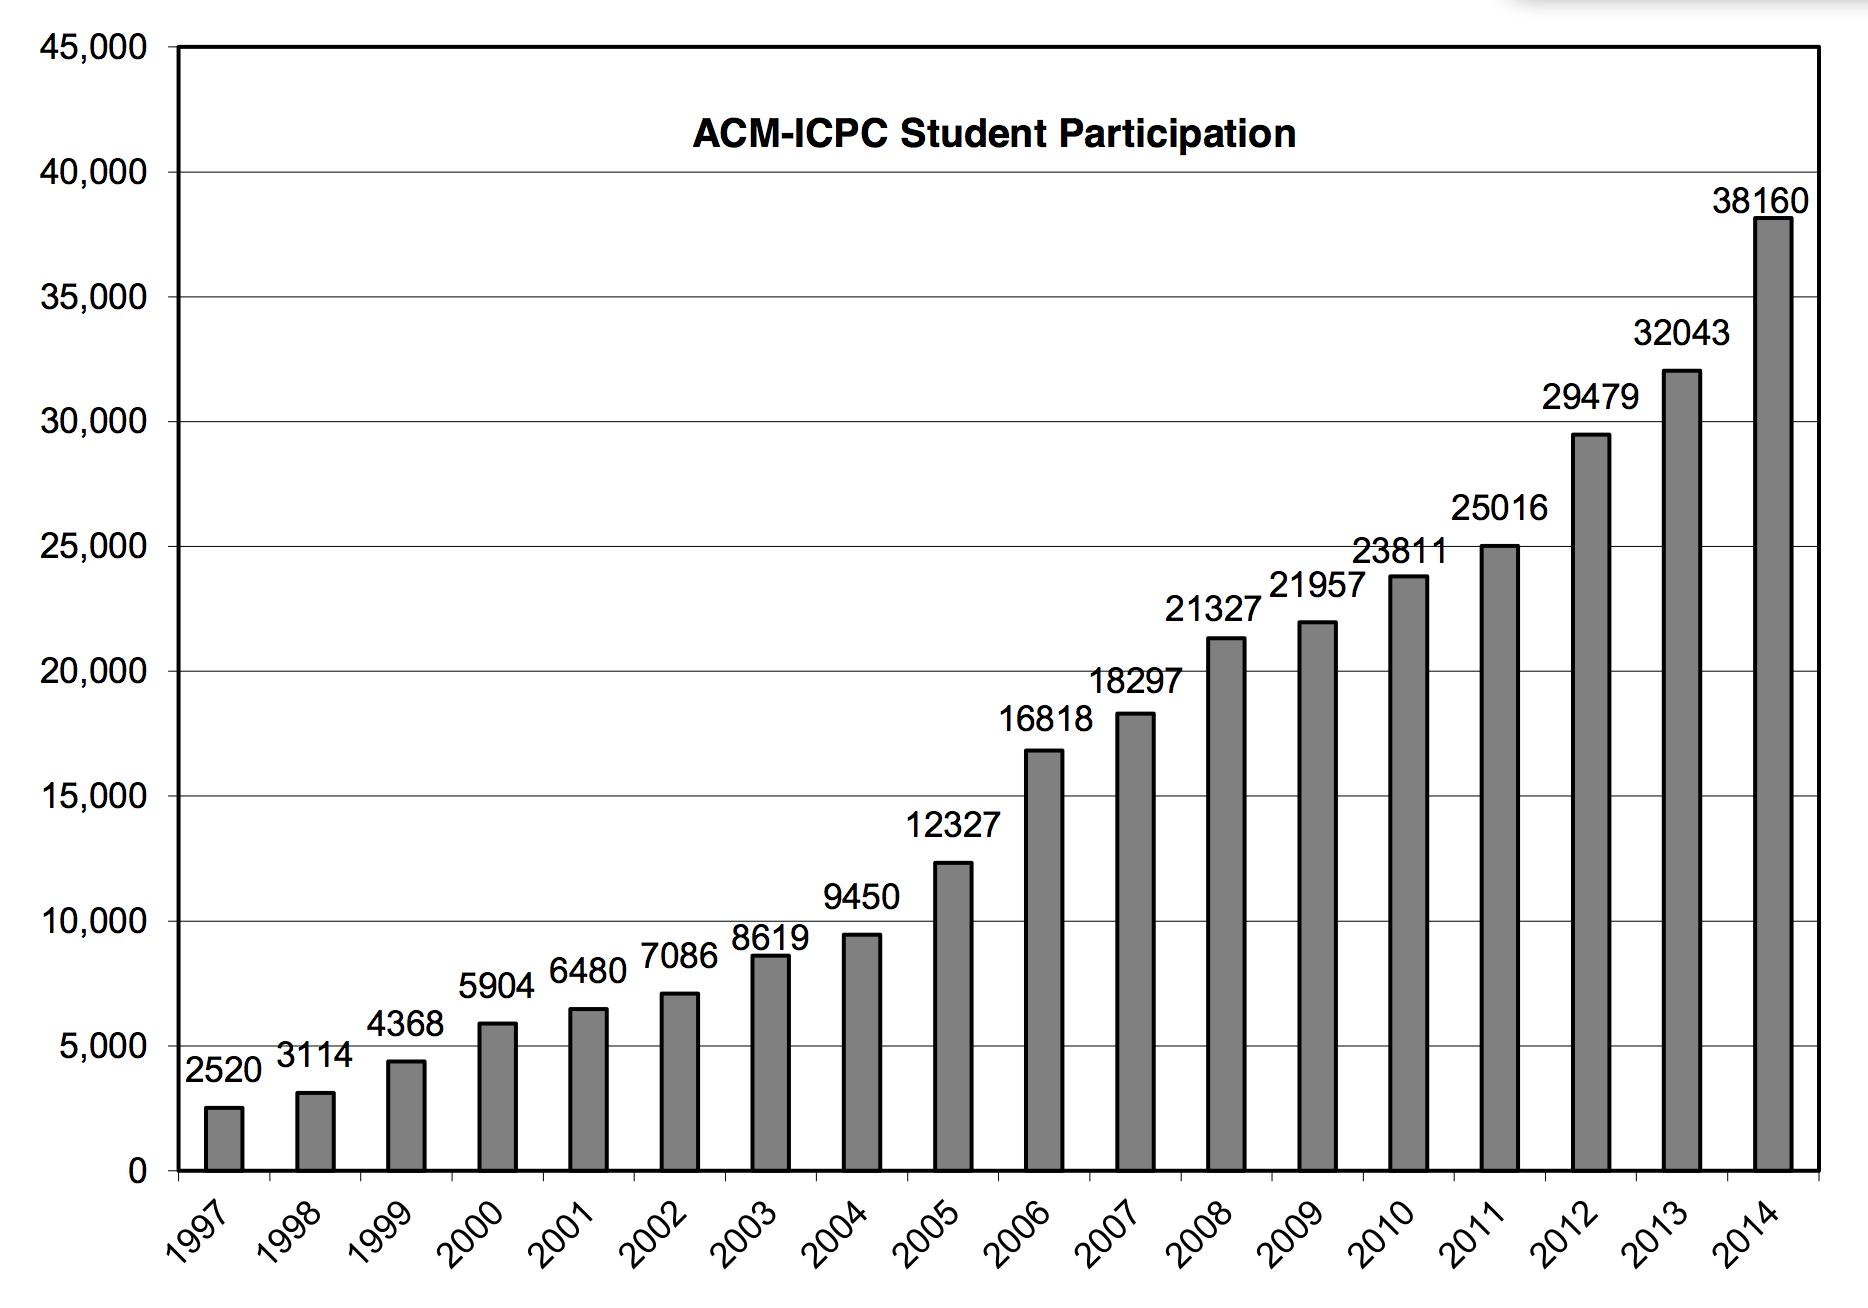
\includegraphics[width=1\linewidth]{Figures/grafico.png}
    \caption{Crescimento do n\'umero de participantes por ano.}
\end{figure}


% Appendix Template

\chapter{Juízes Online (Online Judges)} % Main appendix title

\label{AppendixB} % Change X to a consecutive letter; for referencing this appendix elsewhere, use \ref{AppendixX}

Write your Appendix content here.

%\input{Appendices/AppendixC}

%----------------------------------------------------------------------------------------
%	BIBLIOGRAPHY
%----------------------------------------------------------------------------------------
\clearpage

  \begin{thebibliography}{1}

  \bibitem{notes} OLIVEIRA SANTOS, José Plínio {\em Introdução à Teoria dos Números}  IMPA, 1998. 

	72-85 pg

  \bibitem{notes} CORMEN, Thomas H.; LEISERSON, Charles E.; RIVEST, Ronald L.; STEIN, Clifford {\em Algoritmo Teoria e Prática}  CAMPUS, 2002.
  
  \end{thebibliography}

%\printbibliography[heading=bibintoc]

%----------------------------------------------------------------------------------------

\end{document}  
